\mfpicnumber{1}
\opengraphsfile{IntroRational}

\setcounter{footnote}{0}

\label{IntroRational}

If we add, subtract or multiply polynomial functions according to the function arithmetic rules defined in Section \ref{FunctionArithmetic}, we will produce another polynomial function. If, on the other hand, we divide two polynomial functions, the result may not be a polynomial.  In this chapter we study \index{rational functions} \textbf{rational functions} - functions which are ratios of polynomials.

\smallskip

\colorbox{ResultColor}{\bbm

\begin{defn}  \label{rationalfunction} A \textbf{rational function} is a function which is the ratio of polynomial functions.  Said differently, $r$ is a rational function if it is of the form \index{function ! rational}

\[ r(x) = \dfrac{p(x)}{q(x)},\]

where $p$ and $q$ are polynomial functions.\footnote{According to this definition, all polynomial functions are also  rational functions. (Take $q(x) = 1$).}

\end{defn}

\ebm}

\smallskip

As we recall from Section \ref{FunctionNotation}, we have domain issues anytime the denominator of a fraction is zero.  In the example below, we review this concept as well as some of the arithmetic of rational expressions.

\begin{ex} \label{ratfuncex} Find the domain of the following rational functions.  Write them in the form $\frac{p(x)}{q(x)}$ for polynomial functions $p$ and $q$ and simplify.

\begin{multicols}{2}
\begin{enumerate}

\item  $f(x) = \dfrac{2x-1}{x+1}$
\item  $g(x) = 2 - \dfrac{3}{x+1}$

\setcounter{HW}{\value{enumi}}
\end{enumerate}
\end{multicols}

\begin{multicols}{2}
\begin{enumerate}
\setcounter{enumi}{\value{HW}}

\item  $h(x) = \dfrac{2x^2-1}{x^2-1} - \dfrac{3x-2}{x^2-1}$
\item  $r(x) = \dfrac{2x^2-1}{x^2-1} \div \dfrac{3x-2}{x^2-1}$

\setcounter{HW}{\value{enumi}}
\end{enumerate}
\end{multicols}

{\bf Solution.}

\begin{enumerate}

\item To find the domain of $f$, we proceed as we did in Section \ref{FunctionNotation}: we find the zeros of the denominator and exclude them from the domain.  Setting $x+1=0$ results in  $x=-1$. Hence, our domain is  $(-\infty, -1) \cup (-1,\infty)$.  The expression $f(x)$ is already in the form requested and when we check for common factors among the numerator and denominator we find none, so we are done.

\item  Proceeding as before, we determine the domain of $g$ by solving $x+1=0$.  As before, we find the domain of $g$ is $(-\infty, -1) \cup (-1,\infty)$.  To write $g(x)$ in the form requested, we need to get a common denominator 

\[ \begin{array}{rclclcl}

g(x) & = & 2 - \dfrac{3}{x+1} & = & \dfrac{2}{1} - \dfrac{3}{x+1} & = & \dfrac{(2)(x+1)}{(1)(x+1)} - \dfrac{3}{x+1} \\ [.15in]
     & = & \dfrac{(2x+2) - 3}{x+1} & = & \dfrac{2x-1}{x+1} & & \\ \end{array} \]

This formula is now completely simplified.


\item  The denominators in the formula for $h(x)$ are both $x^2-1$ whose zeros are  $x = \pm 1$.  As a result, the domain of $h$ is $(-\infty, -1) \cup (-1,1) \cup (1, \infty)$.  We now proceed to simplify $h(x)$.  Since we have the same denominator in both terms, we subtract the numerators.  We then factor the resulting numerator and denominator, and cancel out the common factor.

\[ \begin{array}{rclcl}

h(x) & = & \dfrac{2x^2-1}{x^2-1} - \dfrac{3x-2}{x^2-1} & = & \dfrac{\left(2x^2-1\right) - \left(3x-2\right)}{x^2-1} \\ [.15in]
     & = & \dfrac{2x^2-1 - 3x+2}{x^2-1} & = &  \dfrac{2x^2 - 3x+1}{x^2-1} \\ [.15in]
     & = & \dfrac{(2x-1)(x-1)}{(x+1)(x-1)} & = & \dfrac{(2x-1)\cancel{(x-1)}}{(x+1)\cancel{(x-1)}} \\ [.15in]
     & = & \dfrac{2x-1}{x+1} & & \\
\end{array} \]

\item  To find the domain of $r$, it may help to temporarily rewrite $r(x)$ as

\[ r(x) = \dfrac{\dfrac{2x^2-1}{x^2-1} }{\dfrac{3x-2}{x^2-1}\vphantom{\left(\dfrac{X}{X}\right)}}\]

We need to set all of the denominators equal to zero which means we need to solve not only  $x^2-1= 0$, but also $\frac{3x-2}{x^2-1}=0$.  We find $x = \pm 1$ for the former and $x= \frac{2}{3}$ for the latter.  Our domain is $(-\infty, -1) \cup \left(-1,\frac{2}{3}\right) \cup \left(\frac{2}{3},1\right) \cup (1, \infty)$.  We simplify $r(x)$ by rewriting the division as multiplication by the reciprocal and then by canceling the common factor

\[ \begin{array}{rclclcl}

r(x) & = & \dfrac{2x^2-1}{x^2-1} \div \dfrac{3x-2}{x^2-1} & = & \dfrac{2x^2-1}{x^2-1} \cdot \dfrac{x^2-1}{3x-2} & = & \dfrac{\left(2x^2-1\right)\left(x^2-1\right)}{\left(x^2-1\right)(3x-2)} \\ [.15in]
     & = & \dfrac{\left(2x^2-1\right)\cancel{\left(x^2-1\right)}}{\cancel{\left(x^2-1\right)}(3x-2)} & = & \dfrac{2x^2-1}{3x-2} & & \\ 
\end{array}\]

\end{enumerate}

\end{ex}

\vspace{-.35in} \qed

\medskip

A few remarks about Example \ref{ratfuncex} are in order. Note that the expressions for $f(x)$, $g(x)$ and $h(x)$ work out to be the same.  However, only two of these functions are actually equal.  Recall that functions are ultimately sets of ordered pairs,\footnote{You should review Sections \ref{Relations} and \ref{IntrotoFunctions} if this statement caught you off guard.} so for two functions to be equal, they need, among other things, to have the same domain.  Since $f(x) = g(x)$ and $f$ and $g$ have the same domain, they are equal functions.  Even though the formula $h(x)$ is the same as $f(x)$, the domain of $h$ is different than the domain of $f$, and thus they are different functions.  

\medskip

We now turn our attention to the graphs of rational functions. Consider the function $f(x) = \frac{2x-1}{x+1}$ from Example \ref{ratfuncex}.  Using a graphing calculator, we obtain

\medskip

\centerline{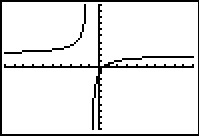
\includegraphics[width=2in]{./RationalsGraphics/Rationals01.jpg}}

\medskip

Two behaviors of the graph are worthy of further discussion.  First, note that the graph appears to `break' at $x=-1$. We know from our last example that $x=-1$ is not in the domain of $f$ which means $f(-1)$ is undefined. When we make a table of values to study the behavior of $f$ \textit{near} $x=-1$ we see that we can get `near' $x=-1$ from two directions.  We can choose values a little less than $-1$, for example $x=-1.1$, $x=-1.01$, $x=-1.001$, and so on.  These values are said to `approach $-1$ from the \textit{left}.'  Similarly, the values $x=-0.9$, $x=-0.99$, $x=-0.999$, etc., are said to `approach $-1$ from the \textit{right}.'  If we make two tables, we find that the numerical results confirm what we see graphically.

\begin{center}
\begin{tabular}{cc}

$\begin{array}{|r||c|c|}  \hline

  x & f(x) & (x,f(x)) \\ \hline
 -1.1 & 32 & (-1.1, 32) \\  \hline
 -1.01 & 302 & (-1.01, 302) \\  \hline 
 -1.001 & 3002 & ( -1.001, 3002) \\  \hline 
  -1.0001 & 30002 & ( -1.001, 30002) \\  \hline 
  \end{array} $ \hspace{.75in} & 

$\begin{array}{|r||c|c|}  \hline 
  x & f(x) & (x,f(x)) \\ \hline
  -0.9 & -28 & ( -0.9 , -28) \\  \hline
  -0.99 & -298 & ( -0.99, -298) \\  \hline
  -0.999 & -2998& (-0.999,-2998) \\  \hline
   -0.9999 & -29998& (-0.9999,-29998) \\  \hline 

\end{array}$

\end{tabular}

\end{center}

As the $x$ values approach $-1$ from the left, the function values become larger and larger positive numbers.\footnote{We would need Calculus to confirm this analytically.}  We express this symbolically by stating as $x \rightarrow -1^{-}$, $f(x) \rightarrow \infty$.   Similarly, using analogous notation, we conclude from the table that as $x \rightarrow -1^{+}$, $f(x) \rightarrow -\infty$.  For this type of unbounded behavior, we say the graph of $y=f(x)$ has a \index{asymptote ! vertical ! intuitive definition of}\index{vertical asymptote ! intuitive definition of}\textbf{vertical asymptote} of $x = -1$.  Roughly speaking, this means that near $x=-1$, the graph looks very much like the vertical line $x=-1$. 

\smallskip

The other feature worthy of note about the graph of $y=f(x)$ is that it seems to `level off' on the left and right hand sides of the screen.  This is a statement about the end behavior of the function.  As we discussed in Section \ref{GraphsofPolynomials}, the end behavior of a function is its behavior as $x$ as $x$ attains larger\footnote{Here, the word `larger' means larger in absolute value.} and larger negative values without bound, $x \rightarrow -\infty$, and as $x$ becomes large without bound, $x \rightarrow \infty$.  Making tables of values, we find

\begin{center}
\begin{tabular}{cc}

$\begin{array}{|r||c|c|}  \hline

  x & f(x) & (x,f(x)) \\ \hline
 -10 & \approx 2.3333 & \approx (-10,  2.3333) \\  \hline
 -100 & \approx 2.0303 & \approx (-100, 2.0303) \\  \hline 
 -1000 &  \approx 2.0030 & \approx ( -1000,  2.0030) \\  \hline 
  -10000 &  \approx 2.0003 & \approx ( -10000, 2.0003) \\  \hline 
  \end{array} $ \hspace{.75in} & 

$\begin{array}{|r||c|c|}  \hline

  x & f(x) & (x,f(x)) \\ \hline
 10 & \approx 1.7273 & \approx (10,  1.7273) \\  \hline
 100 & \approx 1.9703 & \approx (100, 1.9703) \\  \hline 
 1000 &  \approx 1.9970 & \approx ( 1000,  1.9970) \\  \hline 
  10000 &  \approx 1.9997 & \approx ( 10000, 1.9997) \\  \hline 
  \end{array} $  \\

\end{tabular}

\end{center}

From the tables, we see that as $x \rightarrow -\infty$, $f(x) \rightarrow 2^{+}$ and as $x \rightarrow \infty$, $f(x) \rightarrow 2^{-}$.  Here the `$+$' means `from above' and the `$-$' means `from below'.  In this case, we say the graph of $y=f(x)$ has a \index{asymptote ! horizontal ! intuitive definition of}\index{horizontal asymptote ! intuitive definition of}\textbf{horizontal asymptote} of $y=2$.  This means that the end behavior of $f$ resembles the horizontal line $y=2$, which explains the `leveling off' behavior we see in the calculator's graph.  We formalize the concepts of vertical and horizontal asymptotes in the following definitions.

\medskip

\colorbox{ResultColor}{\bbm

\begin{defn} \label{va} The line $x=c$ is called a \index{asymptote ! vertical ! formal definition of}\index{vertical asymptote ! formal definition of}\textbf{vertical asymptote} of the graph of a function $y=f(x)$ if as $x \rightarrow c^{-}$ or as $x \rightarrow c^{+}$, either $f(x) \rightarrow \infty$ or $f(x) \rightarrow -\infty$.

\end{defn}
\ebm}

\medskip

\colorbox{ResultColor}{\bbm

\begin{defn} \label{ha} The line $y=c$ is called a \index{asymptote ! horizontal ! formal definition of}\index{horizontal asymptote ! formal definition of}\textbf{horizontal asymptote} of the graph of a function $y=f(x)$ if as $x \rightarrow -\infty$ or as $x \rightarrow \infty$, $f(x) \rightarrow c$.


\end{defn}
\ebm}

\medskip

Note that in Definition \ref{ha}, we write $f(x) \rightarrow c$ (not $f(x) \rightarrow c^{+}$ or $f(x) \rightarrow c^{-}$) because we are unconcerned from which direction the values $f(x)$ approach the value $c$, just as long as they do so.\footnote{As we shall see in the next section, the graphs of rational functions may, in fact, \textit{cross} their horizontal asymptotes.  If this happens, however,  it does so only a \textit{finite} number of times, and so for each choice of $x \rightarrow -\infty$ and $x \rightarrow \infty$, $f(x)$ will approach $c$ from either below (in the case $f(x) \rightarrow c^{-}$) or above (in the case $f(x) \rightarrow c^{+}$.)  We leave $f(x) \rightarrow c$ generic in our definition, however, to allow this concept to apply to less tame specimens in the Precalculus zoo, such as Exercise \ref{exploregraphslast} in Section \ref{TrigGraphs}.}

In our discussion following Example \ref{ratfuncex}, we determined that, despite the fact that the formula for $h(x)$ reduced to the same formula as $f(x)$, the functions $f$ and $h$ are different, since $x=1$ is in the domain of $f$, but $x=1$ is not in the domain of $h$.  If we graph $h(x)=\frac{2x^2-1}{x^2-1} - \frac{3x-2}{x^2-1}$ using a graphing calculator, we are surprised to find that the graph looks identical to the graph of $y=f(x)$.   There is a vertical asymptote at $x=-1$, but near $x=1$, everything seem fine.  Tables of values provide numerical evidence which supports the graphical observation.

\begin{center}
\begin{tabular}{cc}

$\begin{array}{|r||c|c|}  \hline

  x & h(x) & (x,h(x)) \\ \hline
 0.9 & \approx 0.4210 & \approx (0.9, 0.4210) \\  \hline
 0.99 & \approx 0.4925 & \approx (0.99, 0.4925) \\  \hline
 0.999 & \approx 0.4992 & \approx (0.999, 0.4992) \\  \hline
  0.9999 & \approx 0.4999 & \approx (0.9999, 0.4999) \\  \hline
  \end{array} $ \hspace{.75in} & 

$\begin{array}{|r||c|c|}  \hline 
  x & h(x) & (x,h(x)) \\ \hline
  1.1 & \approx 0.5714 & \approx (1.1, 0.5714) \\  \hline
  1.01 & \approx  0.5075 & \approx (1.01, 0.5075) \\  \hline
  1.001 & \approx 0.5007 & \approx (1.001, 0.5007) \\  \hline
  1.0001 & \approx 0.5001 & \approx (1.0001, 0.5001) \\  \hline

\end{array}$  \\

\end{tabular}

\end{center}

We see that as $x \rightarrow 1^{-}$, $h(x) \rightarrow 0.5^{-}$ and as $x \rightarrow 1^{+}$, $h(x) \rightarrow 0.5^{+}$.  In other words, the points on the graph of $y=h(x)$ are approaching $(1,0.5)$, but since $x=1$ is not in the domain of $h$, it would be inaccurate to fill in a point at $(1,0.5)$.  As we've done in past sections when something like this occurs,\footnote{For instance, graphing piecewise defined functions in Section \ref{GraphsofFunctions}.} we put an open circle (also called a {\bf hole}\index{hole ! in a graph}\index{graph ! hole in} in this case\footnote{In Calculus, we will see how these `holes' can be `plugged' when embarking on a more advanced study of continuity.}) at $(1,0.5)$.  Below is a detailed graph of $y=h(x)$, with the vertical and horizontal asymptotes as dashed lines.

\begin{center}

\begin{mfpic}[15][12]{-5}{5}{-7}{9}
\arrow \reverse \arrow \function{-5,-1.5,0.1}{(2*x-1)/(x+1)}
\arrow \reverse \arrow  \function{-0.63,5,0.1}{(2*x-1)/(x+1)}
\pointfillfalse
\point[3pt]{(1,0.5)}
\dashed \polyline{(-5,2), (5,2)}
\dashed \polyline{(-1,-6), (-1,8)}
\tlabel[cc](5,-0.5){\scriptsize $x$}
\tlabel[cc](0.5,9){\scriptsize $y$}
\axes
\xmarks{-4 step 1 until 4}
\ymarks{-6 step 1 until 8}
\tiny
\tlpointsep{4pt}
\axislabels {x}{ {$-4 \hspace{7pt}$} -4, {$-3\hspace{7pt}$} -3, {$-2\hspace{7pt}$} -2,  {$1$} 1, {$2$} 2, {$3$} 3, {$4$} 4}
\axislabels {y}{ {$\hspace{1in} -1$} -1, {$-2$} -2, {$-3$} -3, {$-4$} -4, {$-5$} -5, {$-6$} -6,  {$1$} 1, {$3$} 3, {$4$} 4, {$5$} 5, {$6$} 6, {$7$} 7, {$8$} 8}
\normalsize
\end{mfpic}

\end{center}
 
Neither $x=-1$ nor $x=1$ are in the domain of $h$, yet the behavior of the graph of $y=h(x)$ is drastically different near these $x$-values.  The reason for this lies in the second to last step when we simplified the formula for $h(x)$ in Example \ref{ratfuncex}, where we had $h(x) = \frac{(2x-1)(x-1)}{(x+1)(x-1)}$.  The reason $x=-1$ is not in the domain of $h$ is because the factor $(x+1)$ appears in the denominator of $h(x)$;  similarly, $x=1$ is not in the domain of $h$ because of the factor $(x-1)$ in the denominator of $h(x)$.  The major difference between these two factors is that $(x-1)$ cancels with a factor in the numerator whereas $(x+1)$ does not.  Loosely speaking, the trouble caused by $(x-1)$ in the denominator is canceled away while the factor $(x+1)$ remains to cause mischief.  This is why the graph of $y=h(x)$ has a vertical asymptote at $x=-1$ but only a hole at $x=1$.  These observations are generalized and summarized in the theorem below, whose proof is found in Calculus.

\smallskip
\colorbox{ResultColor}{\bbm
\begin{thm}  \textbf{Location of Vertical Asymptotes and Holes:}\footnote{Or, `How to tell your asymptote from a hole in the graph.'}  \label{vavshole}  Suppose $r$ is a rational function which can be written as $r(x) = \frac{p(x)}{q(x)}$ where $p$ and $q$ have no common zeros.\footnote{In other words, $r(x)$ is in lowest terms.}  Let $c$ be a real number which is not in the domain of $r$. \index{hole ! location of} \index{asymptote ! vertical ! location of} \index{vertical asymptote ! location of}

\begin{itemize}

\item  If $q(c) \neq 0$, then the graph of $y=r(x)$ has a hole at $\left(c, \frac{p(c)}{q(c)}\right)$.


\item  If $q(c) = 0$, then the line $x=c$ is a vertical asymptote of the graph of $y=r(x)$.



\end{itemize}

\end{thm}

\ebm}

\smallskip

In English,  Theorem \ref{vavshole} says that if $x=c$ is not in the domain of $r$ but, when we simplify $r(x)$,  it no longer makes the denominator $0$, then we have a hole at $x=c$.  Otherwise, the line $x=c$ is a vertical asymptote  of the graph of $y=r(x)$.  

\begin{ex}  \label{vavsholeexample} Find the vertical asymptotes of, and/or holes in, the graphs of the following rational functions.  Verify your answers using a graphing calculator, and describe the behavior of the graph near them using proper notation.

\begin{multicols}{2}
\begin{enumerate}

\item  $f(x) = \dfrac{2x}{x^2-3}$

\item  $g(x) = \dfrac{x^2-x-6}{x^2-9}$

\setcounter{HW}{\value{enumi}}
\end{enumerate}
\end{multicols}

\begin{multicols}{2}
\begin{enumerate}
\setcounter{enumi}{\value{HW}}


\item  $h(x) = \dfrac{x^2-x-6}{x^2+9}$

\item  $r(x) = \dfrac{x^2-x-6}{x^2+4x+4}$

\setcounter{HW}{\value{enumi}}
\end{enumerate}
\end{multicols}


{ \bf Solution.} 

\begin{enumerate}

\item  To use Theorem \ref{vavshole}, we first find all of the real numbers which aren't in the domain of $f$.  To do so, we solve $x^2 - 3 = 0$ and get $x = \pm \sqrt{3}$.  Since the expression $f(x)$ is in lowest terms, there is no cancellation possible, and we conclude that the lines $x = -\sqrt{3}$ and $x=\sqrt{3}$ are vertical asymptotes to the graph of $y=f(x)$.  The calculator verifies this claim, and from the graph, we see that as $x \rightarrow -\sqrt{3}^{\, -}$, $f(x) \rightarrow -\infty$, as $x\rightarrow -\sqrt{3}^{\, +}$, $f(x) \rightarrow \infty$, as $x \rightarrow \sqrt{3}^{\, -}$, $f(x) \rightarrow -\infty$, and finally as $x\rightarrow \sqrt{3}^{\, +}$, $f(x) \rightarrow \infty$.

\item  Solving $x^2 - 9 = 0$ gives $x = \pm 3$.  In lowest terms $g(x) = \frac{x^2-x-6}{x^2-9} = \frac{(x-3)(x+2)}{(x-3)(x+3)} = \frac{x+2}{x+3}$.  Since $x=-3$ continues to make trouble in the denominator, we know the line $x=-3$ is a vertical asymptote of the graph of $y=g(x)$.  Since $x=3$ no longer produces a $0$ in the denominator,  we have a hole at $x=3$.  To find the $y$-coordinate of the hole, we substitute $x=3$ into $\frac{x+2}{x+3}$ and find the hole is at $\left(3, \frac{5}{6}\right)$.  When we graph $y=g(x)$ using a calculator, we clearly see the vertical asymptote at $x=-3$, but everything seems calm near $x=3$.  Hence, as $x \rightarrow -3^{-}$, $g(x) \rightarrow \infty$, as $x \rightarrow -3^{+}$, $g(x) \rightarrow -\infty$, as $x \rightarrow 3^{-}$, $g(x) \rightarrow \frac{5}{6}^{-}$, and as $x \rightarrow 3^{+}$, $g(x) \rightarrow \frac{5}{6}^{+}$.

\begin{center}

\begin{tabular}{cc}

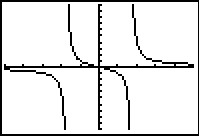
\includegraphics[width=2in]{./RationalsGraphics/Rationals02.jpg} \hspace{0.75in} & 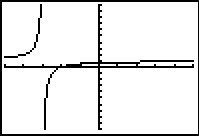
\includegraphics[width=2in]{./RationalsGraphics/Rationals03.jpg} \\

The graph of $y=f(x)$  \hspace{0.75in} & The graph of $y=g(x)$ \\


\end{tabular}
\end{center} 

\item  The domain of $h$ is all real numbers, since $x^2+9 = 0$ has no real solutions.  Accordingly, the graph of $y=h(x)$ is devoid of both vertical asymptotes and holes.

\item  Setting $x^2+4x+4 = 0$ gives us $x=-2$ as the only real number of concern.  Simplifying, we see  $r(x) = \frac{x^2-x-6}{x^2+4x+4} = \frac{(x-3)(x+2)}{(x+2)^2} = \frac{x-3}{x+2}$.  Since $x=-2$ continues to produce a $0$ in the denominator of the reduced function, we know $x=-2$ is a vertical asymptote to the graph.  The calculator bears this out, and, moreover, we see that as $x\rightarrow -2^{-}$, $r(x) \rightarrow \infty$ and as $x \rightarrow -2^{+}$, $r(x) \rightarrow -\infty$.


\begin{center}

\begin{tabular}{cc}

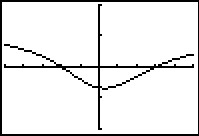
\includegraphics[width=2in]{./RationalsGraphics/Rationals04.jpg} \hspace{0.75in} & 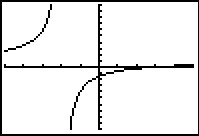
\includegraphics[width=2in]{./RationalsGraphics/Rationals05.jpg} \\

The graph of $y=h(x)$  \hspace{0.75in} & The graph of $y=r(x)$ \\


\end{tabular}
\end{center} 

\end{enumerate}
\qed
\end{ex}

Our next example gives us a physical interpretation of a vertical asymptote.  This type of model arises from a family of equations cheerily named `doomsday' equations.\footnote{These functions arise in Differential Equations.  The unfortunate name will make sense shortly.}  

\begin{ex}  A mathematical model for the population $P$, in thousands, of a certain species of bacteria, $t$ days after it is introduced to an environment is given by $P(t) = \frac{100}{(5-t)^{2}}$, $0 \leq t < 5$.


\begin{enumerate}

\item  Find and interpret $P(0)$.

\item  When will the population reach $100,\!000$?

\item  Determine the behavior of $P$ as $t \rightarrow 5^{-}$.  Interpret this result graphically and within the context of the problem. 

\end{enumerate}

{ \bf Solution.}  

\begin{enumerate}

\item  Substituting $t=0$ gives $P(0) = \frac{100}{(5-0)^2} = 4$, which means $4000$ bacteria are initially introduced into the environment.

\item  To find when the population reaches $100,\! 000$, we first need to remember that $P(t)$ is measured in \textit{thousands}.  In other words, $100,\! 000$ bacteria corresponds to $P(t) = 100$.  Substituting for $P(t)$ gives the equation  $\frac{100}{(5-t)^2} = 100$.  Clearing denominators and dividing by $100$ gives $(5-t)^2=1$, which, after extracting square roots, produces $t = 4$ or $t=6$.  Of these two solutions, only $t=4$ in in our domain, so this is the solution we keep.  Hence, it takes $4$ days for the population of bacteria to reach $100,\! 000$.

\item To determine the behavior of $P$ as $t \rightarrow 5^{-}$, we can make a table

\[\begin{array}{|r||c|}  \hline

  t & P(t)  \\ \hline
 4.9 & 10000  \\  \hline
 4.99 & 1000000  \\  \hline
 4.999 &  100000000  \\  \hline
  4.9999 & 10000000000  \\  \hline
  \end{array}\]

In other words, as $t \rightarrow 5^{-}$, $P(t) \rightarrow \infty$.  Graphically, the line $t=5$ is a vertical asymptote of the graph of $y=P(t)$.  Physically, this means that the population of bacteria is increasing without bound as we near 5 days, which cannot actually happen.  For this reason, $t=5$ is called the `doomsday' for this population. There is no way any environment can support infinitely many bacteria, so shortly before $t = 5$ the environment would collapse. \qed

\end{enumerate}

Now that we have thoroughly investigated vertical asymptotes, we can turn our attention to horizontal asymptotes.  The next theorem tells us when to expect horizontal asymptotes.

\smallskip
\colorbox{ResultColor}{\bbm

\begin{thm} \index{asymptote ! horizontal ! location of}\index{horizontal asymptote ! location of}\textbf{Location of Horizontal Asymptotes:}\label{hathm} Suppose $r$ is a rational function and $r(x) = \frac{p(x)}{q(x)}$, where $p$ and $q$ are polynomial functions with leading coefficients $a$ and $b$, respectively. 

\begin{itemize}

\item  If the degree of $p(x)$ is the same as the degree of $q(x)$, then $y=\frac{a}{b}$ is the\footnote{The use of the definite article will be justified momentarily.} horizontal asymptote of the graph of $y=r(x)$.

\item  If the degree of $p(x)$ is less than the degree of $q(x)$, then $y=0$ is the horizontal asymptote of the graph of $y=r(x)$.

\item  If the degree of $p(x)$ is greater than the degree of $q(x)$, then the graph of $y=r(x)$ has no horizontal asymptotes.


\end{itemize}
\end{thm}
\ebm}
\smallskip

\end{ex}

Like Theorem \ref{vavshole}, Theorem \ref{hathm} is proved using Calculus.  Nevertheless, we can understand the idea behind it using our example $f(x) = \frac{2x-1}{x+1}$.  If we interpret $f(x)$ as a division problem, $(2x-1) \div (x+1)$, we find that the quotient is $2$ with a remainder of $-3$.  Using what we know about polynomial division, specifically Theorem \ref{polydiv}, we get $2x-1 = 2(x+1) -3$.  Dividing both sides by $(x+1)$ gives   $\frac{2x-1}{x+1} = 2 - \frac{3}{x+1}$.  (You may remember this as the formula for $g(x)$ in Example \ref{ratfuncex}.)  As $x$ becomes unbounded in either direction, the quantity $\frac{3}{x+1}$ gets closer and closer to $0$ so that the values of $f(x)$ become closer and closer\footnote{As seen in the tables immediately preceding Definition \ref{va}.} to $2$. In symbols, as $x \rightarrow \pm \infty$, $f(x) \rightarrow 2$, and we have the result.\footnote{More specifically, as $x \rightarrow -\infty$, $f(x) \rightarrow 2^{+}$, and as $x \rightarrow \infty$, $f(x) \rightarrow 2^{-}$.}  Notice that the graph gets close to the same $y$ value as $x \rightarrow -\infty$ or $x \rightarrow \infty$.  This means that the graph can have only \underline{one} horizontal asymptote if it is going to have one at all.  Thus we were justified in using `the' in the previous theorem.

\smallskip

Alternatively, we can use what we know about end behavior of polynomials to help us understand this theorem.  From Theorem \ref{EBPolynomials}, we know the end behavior of a polynomial is determined by its leading term.  Applying this to the numerator and denominator of $f(x)$, we get that as $x \rightarrow \pm \infty$, $f(x) = \frac{2x-1}{x+1} \approx \frac{2x}{x} = 2$.  This last approach is useful in Calculus, and, indeed, is made rigorous there.  (Keep this in mind for the remainder of this paragraph.)  Applying this reasoning to the general case, suppose $r(x) = \frac{p(x)}{q(x)}$ where $a$ is the leading coefficient of $p(x)$ and $b$ is the leading coefficient of $q(x)$. As $x \rightarrow \pm \infty$, $r(x) \approx \frac{ax^n}{bx^m}$, where $n$ and $m$ are the degrees of $p(x)$ and $q(x)$, respectively.  If the degree of $p(x)$ and the degree of $q(x)$ are the same, then $n=m$ so that $r(x) \approx \frac{a}{b}$, which means $y=\frac{a}{b}$ is the horizontal asymptote in this case.  If the degree of $p(x)$ is less than the degree of $q(x)$, then $n < m$, so $m-n$ is a positive number, and hence, $r(x) \approx \frac{a}{bx^{m-n}} \rightarrow 0$ as $x \rightarrow \pm \infty$.  If the degree of $p(x)$ is greater than the degree of $q(x)$, then $n > m$, and hence $n-m$ is a positive number and $r(x) \approx \frac{ax^{n-m}}{ b}$, which becomes unbounded as $x \rightarrow \pm \infty$.  As we said before, if a rational function has a horizontal asymptote, then it will have only one.  (This is not true for other types of functions we shall see in later chapters.)
 
\begin{ex} \label{haexample} List the horizontal asymptotes, if any, of the graphs of the following functions.  Verify your answers using a graphing calculator, and describe the behavior of the graph near them using proper notation.

\begin{multicols}{3}

\begin{enumerate}

\item $f(x) = \dfrac{5x}{x^2+1}$  

\item  $g(x) = \dfrac{x^2-4}{x+1}$

\item  $h(x) = \dfrac{6x^3-3x+1}{5-2x^3}$

\end{enumerate}

\end{multicols}

{ \bf Solution.}

\begin{enumerate}

\item  The numerator of $f(x)$ is $5x$, which has degree $1$.  The denominator of $f(x)$ is $x^2+1$, which has degree $2$.  Applying Theorem \ref{hathm},  $y=0$ is the horizontal asymptote.  Sure enough, we see from the graph that as $x \rightarrow - \infty$, $f(x) \rightarrow 0^{-}$ and as $x \rightarrow \infty$, $f(x) \rightarrow 0^{+}$.

\item  The numerator of $g(x)$, $x^2-4$, has degree $2$, but the degree of the denominator, $x+1$, has degree $1$.  By Theorem \ref{hathm}, there is no horizontal asymptote.  From the graph, we see that the graph of $y=g(x)$ doesn't appear to level off to a constant value, so there is no horizontal asymptote.\footnote{Sit tight!  We'll revisit this function and its end behavior shortly.}

\item  The degrees of the numerator and denominator of $h(x)$ are both three, so Theorem \ref{hathm} tells us $y = \frac{6}{-2} = -3$ is the horizontal asymptote.  We see from the calculator's graph that as $x \rightarrow -\infty$, $h(x) \rightarrow -3^{+}$, and as $x \rightarrow \infty$, $h(x) \rightarrow -3^{-}$.

\begin{center}

\begin{tabular}{ccc}

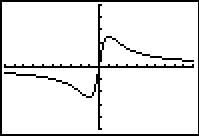
\includegraphics[width=1.75in]{./RationalsGraphics/Rationals06.jpg}  & 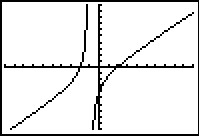
\includegraphics[width=1.75in]{./RationalsGraphics/Rationals07.jpg} & 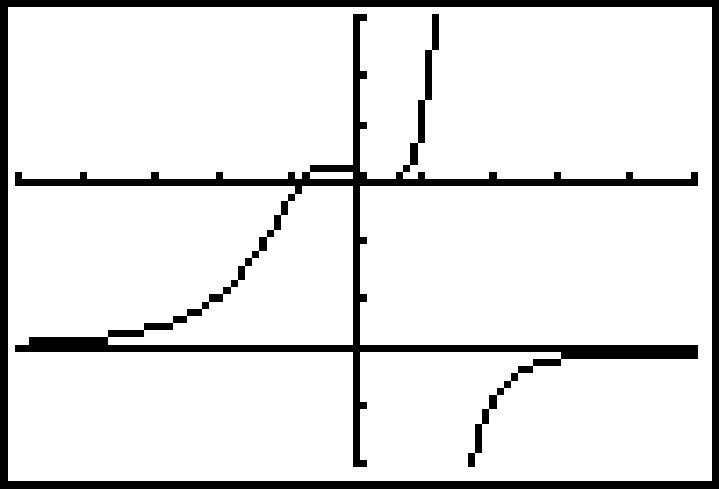
\includegraphics[width=1.75in]{./RationalsGraphics/Rationals08.jpg} \\

The graph of $y=f(x)$  & The graph of $y=g(x)$ & The graph of $y=h(x)$ \\


\end{tabular}
\end{center} 

\end{enumerate}

\vspace{-.25in} \qed

\end{ex}

Our next example of the section gives us a real-world application of a horizontal asymptote.\footnote{Though the population below is more accurately modeled with the functions in Chapter \ref{ExpLogs}, we approximate it (using Calculus, of course!) using a rational function.}

\begin{ex}  The number of students $N$ at local college who have had the flu $t$ months after the semester begins can be modeled by the formula $N(t) = 500 - \frac{450}{1+3t}$ for $t \geq 0$.

\begin{enumerate}

\item  Find and interpret $N(0)$.

\item  How long will it take until $300$ students will have had the flu?

\item  Determine the behavior of $N$ as $t \rightarrow \infty$.  Interpret this result graphically and within the context of the problem. 

\end{enumerate}

{ \bf Solution.}

\begin{enumerate}

\item  $N(0) = 500 - \frac{450}{1+3(0)} = 50$.  This means that at the beginning of the semester, $50$ students have had the flu.

\item  We set $N(t) = 300$ to get $500 - \frac{450}{1+3t} = 300$ and solve.  Isolating the fraction gives $\frac{450}{1+3t} = 200$.  Clearing denominators gives $450 = 200(1+3t)$.  Finally, we get $t = \frac{5}{12}$.  This means it will take $\frac{5}{12}$ months, or about 13 days, for $300$ students to have had the flu.

\item  To determine the behavior of $N$ as $t\rightarrow \infty$, we can use a table. 


\[\begin{array}{|r||c|}  \hline

  t & N(t)  \\ \hline
 10 & \approx 485.48  \\  \hline
 100& \approx 498.50  \\  \hline
 1000 &  \approx 499.85  \\  \hline
  10000 & \approx 499.98  \\  \hline
  \end{array}\]
  
The table suggests that as $t \rightarrow \infty$, $N(t) \rightarrow 500$. (More specifically, $500^{-}$.)  This means as time goes by, only a total of 500 students will have ever had the flu. \qed

\end{enumerate}

\end{ex}

We close this section with a discussion of the \textit{third} (and final!) kind of asymptote which can be associated with the graphs of rational functions. Let us return to the function $g(x) = \frac{x^2-4}{x+1}$ in Example \ref{haexample}. Performing long division,\footnote{See the remarks following Theorem \ref{hathm}.} we get $g(x) = \frac{x^2-4}{x+1} = x-1 - \frac{3}{x+1}$.  Since the term $\frac{3}{x+1} \rightarrow 0$ as $x \rightarrow \pm \infty$, it stands to reason that as $x$ becomes unbounded, the function values   $g(x) = x-1 - \frac{3}{x+1} \approx x-1$.  Geometrically, this means that the graph of $y=g(x)$ should resemble the line $y = x-1$ as $x \rightarrow \pm \infty$.  We see this play out both numerically and graphically below.

\begin{center}
\begin{tabular}{cc}

$\begin{array}{|r||c|c|}  \hline

  x & g(x) & x-1 \\ \hline
 -10 & \approx -10.6667 & -11 \\  \hline
 -100 & \approx -100.9697 & -101 \\  \hline 
 -1000 &  \approx -1000.9970&   -1001 \\ \hline 
  -10000 &  \approx -10000.9997 &  -10001 \\ \hline 
  \end{array} $ & \hspace{0.75in}

$\begin{array}{|r||c|c|}  \hline

  x & g(x) & x-1 \\ \hline
 10 & \approx 8.7273 &    9 \\\hline
 100 & \approx 98.9703 &   99 \\ \hline 
 1000 &  \approx 998.9970 &  999 \\ \hline 
  10000 &  \approx 9998.9997 &   9999 \\ \hline 
  \end{array} $ \\ 
  
  & \\
  
  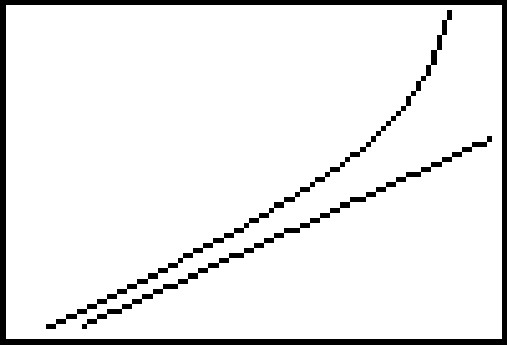
\includegraphics[width=2in]{./RationalsGraphics/SA01.jpg} & \hspace{0.75in}
  
  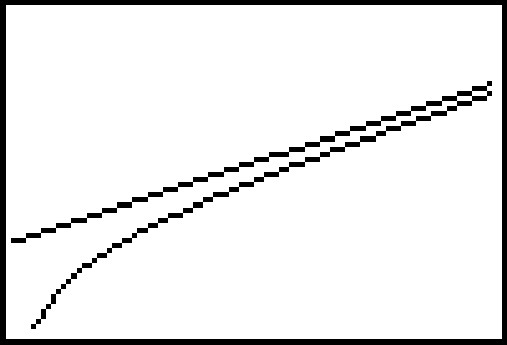
\includegraphics[width=2in]{./RationalsGraphics/SA02.jpg} \\
  
   $y= g(x)$ and $y=x-1$ & \hspace{0.75in} $y = g(x)$ and $y=x-1$ \\
    as $x \rightarrow -\infty$ & \hspace{0.75in} as $x \rightarrow \infty$ \\

\end{tabular}

\end{center}

The way we symbolize the relationship between the end behavior of $y=g(x)$ with that of the line $y=x-1$ is to write `as $x \rightarrow \pm \infty$, $g(x) \rightarrow x-1$.'  In this case, we say the line $y=x-1$ is a \index{asymptote ! slant (oblique)} \index{slant asymptote} \index{oblique asymptote} \textbf{slant asymptote}\footnote{Also called an `oblique' asymptote in some, ostensibly higher class (and more expensive), texts.}  to the graph of $y=g(x)$.  Informally, the graph of a rational function has a slant asymptote if, as $x \rightarrow \infty$ or as $x \rightarrow -\infty$, the graph resembles a non-horizontal, or `slanted' line.  Formally, we define a slant asymptote as follows.


\medskip


\colorbox{ResultColor}{\bbm

\begin{defn} \label{sa} The line $y = mx+b$ where $m \neq 0$  is called a \index{asymptote ! slant ! formal definition of}\index{slant asymptote ! formal definition of}\textbf{slant asymptote} of the graph of a function $y=f(x)$ if as $x \rightarrow -\infty$ or as $x \rightarrow \infty$, $f(x)  \rightarrow mx+b$.


\end{defn}
\ebm}

\medskip


A few remarks are in order.  First, note that the stipulation $m \neq 0$ in Definition \ref{sa} is what makes the `slant' asymptote `slanted' as opposed to the case when $m=0$ in which case we'd have a horizontal asymptote.  Secondly, while we have motivated what me mean intuitively by the notation `$f(x)  \rightarrow mx+b$,' like so many ideas in this section, the formal definition requires Calculus.  Another way to express this sentiment, however, is to rephrase `$f(x)  \rightarrow mx+b$' as `$f(x) - (mx+b) \rightarrow 0$.'  In other words, the graph of $y=f(x)$ has the \textit{slant} asymptote $y = mx+b$ if and only if the graph of $y = f(x) - (mx+b)$ has a \textit{horizontal} asymptote $y=0$.


Our next task is to determine the conditions under which the graph of a rational function has a slant asymptote, and if it does, how to find it.  In the case of $g(x) = \frac{x^2-4}{x+1}$, the degree of the numerator $x^2-4$ is $2$, which is \textit{exactly one more} than the degree if its denominator $x+1$ which is $1$.  This results in a \textit{linear} quotient polynomial, and it is this quotient polynomial which is the slant asymptote.  Generalizing this situation gives us the following theorem.\footnote{Once again, this theorem is brought to you courtesy of Theorem \ref{polydiv} and Calculus.}

\medskip

\colorbox{ResultColor}{\bbm

\begin{thm} \textbf{Determination of Slant Asymptotes:} \label{sathm} Suppose $r$ is a rational function and $r(x) = \frac{p(x)}{q(x)}$, where the degree of $p$ is \textit{exactly} one more than the degree of $q$.  Then the graph of $y=r(x)$ has \index{asymptote ! slant ! determination of}\index{slant asymptote ! determination of} the slant asymptote $y=L(x)$ where $L(x)$ is the quotient obtained by dividing $p(x)$ by $q(x)$.

\end{thm}
\ebm}

\medskip

In the same way that Theorem \ref{hathm} gives us an easy way to see if the graph of a rational function $r(x) = \frac{p(x)}{q(x)}$ has a horizontal asymptote by comparing the degrees of the numerator and denominator, Theorem \ref{sathm} gives us an easy way to check for slant asymptotes.  Unlike Theorem \ref{hathm}, which gives us a quick way to \textit{find} the horizontal asymptotes (if any exist), Theorem \ref{sathm} gives us no such `short-cut'.  If a slant asymptote exists, we have no recourse but to use long division to find it.\footnote{That's OK, though.  In the next section, we'll use long division to analyze end behavior and it's worth the effort!}  

\begin{ex} \label{saexample} Find the slant asymptotes of the graphs of the following functions if they exist.  Verify your answers using a graphing calculator and describe the behavior of the graph near them using proper notation.

\begin{multicols}{3}

\begin{enumerate}

\item  $f(x) = \dfrac{x^2-4x+2}{1-x}$  

\item  \label{sacancel} $g(x) = \dfrac{x^2-4}{x-2}$

\item  $h(x) = \dfrac{x^3+1}{x^2-4}$

\end{enumerate}

\end{multicols}


{\bf Solution.}

\begin{enumerate}

\item  The degree of the numerator is $2$ and the degree of the denominator is $1$, so Theorem \ref{sathm} guarantees us a slant asymptote.  To find it, we divide $1-x = -x+1$ into $x^2-4x+2$ and get a quotient of $-x+3$, so our slant asymptote is $y=-x+3$.  We confirm this graphically, and we see that as $x \rightarrow -\infty$, the graph of $y=f(x)$ approaches the asymptote from below, and as $x \rightarrow \infty$, the graph of $y=f(x)$ approaches the asymptote from above.\footnote{Note that we are purposefully avoiding notation like `as $x\rightarrow \infty$, $f(x) \rightarrow (-x+3)^{+}$.  While it is possible to define these notions formally with Calculus, it is not standard to do so.  Besides, with the introduction of the symbol `\textinterrobang' in the next section, the authors feel we are in enough trouble already.}

\item  As with the previous example, the degree of the numerator $g(x) = \frac{x^2-4}{x-2}$ is $2$ and the degree of the denominator is $1$, so Theorem \ref{sathm} applies.  In this case, 

\[ g(x) = \frac{x^2-4}{x-2} = \frac{(x+2)(x-2)}{(x-2)} = \frac{(x+2) \cancel{(x-2)}}{\cancelto{1}{(x-2)}} = x+2, \quad x \neq 2\]

so we have that the slant asymptote $y=x+2$ is identical to the graph of $y=g(x)$ except at $x=2$ (where the latter has a `hole' at $(2,4)$.)  The calculator supports this claim.\footnote{While the word `asymptote' has the connotation of `approaching but not equaling,' Definitions \ref{ha} and \ref{sa} invite the same kind of pathologies we saw with Definitions \ref{maxmindefn} in Section \ref{GraphsofFunctions}.}

\item   For $h(x) = \frac{x^3+1}{x^2-4}$, the degree of the numerator is $3$ and the degree of the denominator is $2$ so again, we are guaranteed the existence of a slant asymptote.  The long division $\left(x^3+1 \right) \div \left(x^2-4\right)$ gives a quotient of just $x$, so our slant asymptote is the line $y=x$.  The calculator confirms this, and we find that as $x \rightarrow -\infty$, the graph of $y=h(x)$ approaches the asymptote from below, and as $x \rightarrow \infty$, the graph of $y=h(x)$ approaches the asymptote from above. 

\begin{center}

\begin{tabular}{ccc}

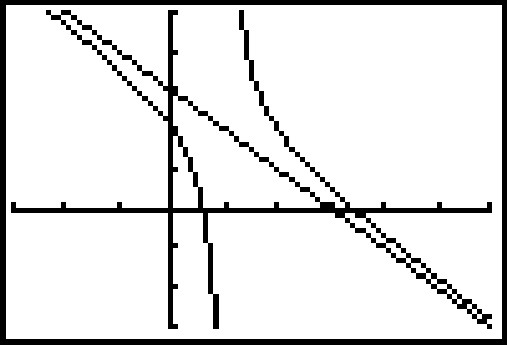
\includegraphics[width=1.75in]{./RationalsGraphics/SAEX01.jpg}  & 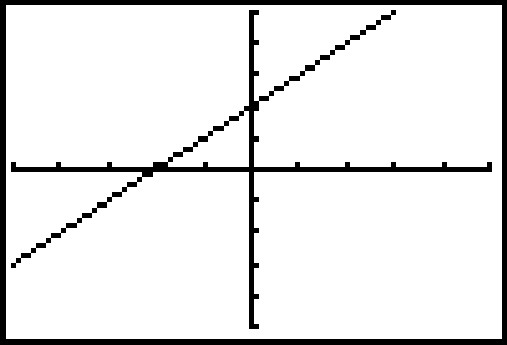
\includegraphics[width=1.75in]{./RationalsGraphics/SAEX02.jpg} & 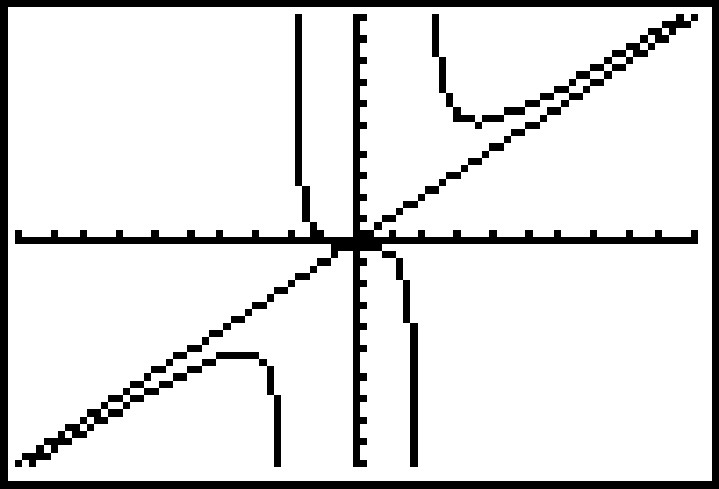
\includegraphics[width=1.75in]{./RationalsGraphics/SAEX03.jpg} \\

The graph of $y=f(x)$  & The graph of $y=g(x)$ & The graph of $y=h(x)$ \\


\end{tabular}
\end{center} 


\qed

\end{enumerate}

\end{ex}



The reader may be a bit disappointed with the authors at this point owing to the fact that in Examples \ref{vavsholeexample}, \ref{haexample}, and \ref{saexample}, we used the \textit{calculator} to determine function behavior near asymptotes.  We rectify that in the next section where we, in excruciating detail, demonstrate the usefulness of `number sense' to reveal this behavior analytically.  
\newpage

\subsection{Exercises}

In Exercises \ref{alltheasympfirst} - \ref{alltheasymplast}, for the given rational function $f$:

\begin{itemize}

\item Find the domain of $f$.
\item Identify any vertical asymptotes of the graph of $y = f(x)$.
\item Identify any holes in the graph.
\item Find the horizontal asymptote, if it exists.
\item Find the slant asymptote, if it exists.
\item Graph the function using a graphing utility and describe the behavior near the asymptotes.

\end{itemize}

\begin{multicols}{3}
\begin{enumerate}

\item $f(x) = \dfrac{x}{3x - 6}$ \label{alltheasympfirst}
\item $f(x) = \dfrac{3 + 7x}{5 - 2x}$
\item $f(x) = \dfrac{x}{x^{2} + x - 12}$

\setcounter{HW}{\value{enumi}}
\end{enumerate}
\end{multicols}

\begin{multicols}{3}
\begin{enumerate}
\setcounter{enumi}{\value{HW}}

\item $f(x) = \dfrac{x}{x^{2} + 1}$
\item $f(x) = \dfrac{x + 7}{(x + 3)^{2}}$
\item $f(x) = \dfrac{x^{3} + 1}{x^{2} - 1}$

\setcounter{HW}{\value{enumi}}
\end{enumerate}
\end{multicols}

\begin{multicols}{3}
\begin{enumerate}
\setcounter{enumi}{\value{HW}}

\item $f(x) = \dfrac{4x}{x^2+4}$
\item $f(x) = \dfrac{4x}{x^2-4}$
\item $f(x) = \dfrac{x^2-x-12}{x^2+x-6}$

\setcounter{HW}{\value{enumi}}
\end{enumerate}
\end{multicols}

\begin{multicols}{3}
\begin{enumerate}
\setcounter{enumi}{\value{HW}}

\item $f(x) = \dfrac{3x^2-5x-2}{x^2-9}$
\item $f(x) = \dfrac{x^3+2x^2+x}{x^2-x-2}$
\item $f(x) = \dfrac{x^{3} - 3x + 1}{x^{2} + 1}$

\setcounter{HW}{\value{enumi}}
\end{enumerate}
\end{multicols}

\begin{multicols}{3}
\begin{enumerate}
\setcounter{enumi}{\value{HW}}

\item $f(x) = \dfrac{2x^{2} + 5x - 3}{3x + 2}$
\item $f(x) = \dfrac{-x^{3} + 4x}{x^{2} - 9}$
\item \small $f(x) = \dfrac{-5x^{4} - 3x^{3} + x^{2} - 10}{x^{3} - 3x^{2} + 3x - 1}$ \normalsize 

\setcounter{HW}{\value{enumi}}
\end{enumerate}
\end{multicols}


\begin{multicols}{3}
\begin{enumerate}
\setcounter{enumi}{\value{HW}}

\item $f(x) = \dfrac{x^3}{1-x}$
\item $f(x) = \dfrac{18-2x^2}{x^2-9}$
\item $f(x) = \dfrac{x^3-4x^2-4x-5}{x^2+x+1}$ \label{alltheasymplast}


\setcounter{HW}{\value{enumi}}
\end{enumerate}
\end{multicols}

\begin{enumerate}
\setcounter{enumi}{\value{HW}}

\item The cost $C$ in dollars to remove $p$\% of the invasive species of Ippizuti fish from Sasquatch Pond is given by \[C(p) = \frac{1770p}{100 - p}, \quad 0 \leq p < 100 \]

\begin{enumerate}

\item Find and interpret $C(25)$ and $C(95)$.
\item What does the vertical asymptote at $x = 100$ mean within the context of the problem?  
\item What percentage of the Ippizuti fish can you remove for  \$40000?

\end{enumerate}


\item In Exercise \ref{Sasquatchfunc1} in Section \ref{FunctionNotation}, the population of Sasquatch in Portage County was modeled by the function \[P(t) = \frac{150t}{t + 15},\] where $t = 0$ represents the year 1803.  Find the horizontal asymptote of the graph of $y = P(t)$ and explain what it means.

\item  Recall from Example \ref{costrevenueprofitex1} that the cost $C$ (in dollars) to make $x$ dOpi media players is $C(x) = 100x+2000$, $x \geq 0$.  

\begin{enumerate}

\item  Find a formula for the average cost $\overline{C}(x)$. Recall:  $\overline{C}(x) = \frac{C(x)}{x}$.

\item  Find and interpret $\overline{C}(1)$ and $\overline{C}(100)$.

\item  How many dOpis need to be produced so that the average cost per dOpi is $\$ 200$?

\item  Interpret the behavior of $\overline{C}(x)$ as $x \rightarrow 0^{+}$.  (HINT:  You may want to find the fixed cost $C(0)$ to help in your interpretation.)

\item  Interpret the behavior of $\overline{C}(x)$ as $x \rightarrow \infty$.  (HINT:  You may want to find the variable cost (defined in Example \ref{PortaBoyCost} in Section \ref{LinearFunctions}) to help in your interpretation.)


\end{enumerate}

\item In Exercise \ref{circuitexercisepoly} in Section \ref{GraphsofPolynomials}, we fit a few polynomial models to the following electric circuit data. (The circuit was built with a variable resistor.  For each of the following resistance values (measured in kilo-ohms, $k \Omega$),  the corresponding power to the load (measured in milliwatts, $mW$) is given in the table below.)\footnote{The authors wish to thank Don Anthan and Ken White of Lakeland Community College for devising this problem and generating the accompanying data set.}


\smallskip

\noindent \begin{tabular}{|l|r|r|r|r|r|r|} \hline
Resistance: ($k \Omega$) & 1.012 & 2.199 & 3.275 & 4.676 & 6.805 & 9.975 \\ \hline
Power: ($mW$) & 1.063 & 1.496 & 1.610 & 1.613 & 1.505 & 1.314 \\ \hline
\end{tabular}

\smallskip

\noindent Using some fundamental laws of circuit analysis mixed with a healthy dose of algebra, we can derive the actual formula relating power to resistance.  For this circuit, it is $P(x) = \frac{25x}{(x + 3.9)^2}$, where $x$ is the resistance value, $x \geq 0$.

\begin{enumerate}

\item Graph the data along with the function $y = P(x)$ on your calculator.

\item Use your calculator to approximate the maximum power that can be delivered to the load.  What is the corresponding resistance value?

\item Find and interpret the end behavior of $P(x)$ as $x \rightarrow \infty$.

\end{enumerate}

\item \index{Learning Curve Equation} \index{Thurstone, Louis Leon} In his now famous 1919 dissertation \underline{The Learning Curve Equation}, Louis Leon Thurstone presents a rational function which models the number of words a person can type in four minutes as a function of the number of pages of practice one has completed.  (This paper, which is now in the public domain and can be found  \href{http://books.google.com/books?id=pb5BAAAAIAAJ&dq=Louis+Leon+Thurstone&printsec=frontcover&source=an&hl=en&ei=Ev_bSaeKGInEMbmM9OQN&sa=X&oi=book_result&ct=result&resnum=6#PPP1,M1}{\underline{here}}, is from a bygone era when students at business schools took typing classes on manual typewriters.)  Using his original notation and original language, we have $Y = \frac{L(X + P)}{(X + P) + R}$ where $L$ is the predicted practice limit in terms of speed units, $X$ is pages written, $Y$ is writing speed in terms of words in four minutes, $P$ is equivalent previous practice in terms of pages and $R$ is the rate of learning. In Figure 5 of the paper, he graphs a scatter plot and the curve $Y = \frac{216(X + 19)}{X + 148}$.  Discuss this equation with your classmates.  How would you update the notation?  Explain what the horizontal asymptote of the graph means.  You should take some time to look at the original paper. Skip over the computations you don't understand yet and try to get a sense of the time and place in which the study was conducted.

\end{enumerate}

\newpage

\subsection{Answers}

\begin{multicols}{2}
\begin{enumerate} 

\item $f(x) = \dfrac{x}{3x - 6}$ \vphantom{$\dfrac{7x}{7x}$}\\ 
Domain: $(-\infty, 2) \cup (2, \infty)$\\
Vertical asymptote: $x = 2$\\
As $x \rightarrow 2^{-}, f(x) \rightarrow -\infty$\\
As $x \rightarrow 2^{+}, f(x) \rightarrow \infty$\\
No holes in the graph\\
Horizontal asymptote: $y = \frac{1}{3}$ \\
As $x \rightarrow -\infty, f(x) \rightarrow \frac{1}{3}^{-}$\\
As $x \rightarrow \infty, f(x) \rightarrow \frac{1}{3}^{+}$\\

\vfill

\columnbreak

\item $f(x) = \dfrac{3 + 7x}{5 - 2x}$\\
Domain: $(-\infty, \frac{5}{2}) \cup (\frac{5}{2}, \infty)$\\
Vertical asymptote: $x = \frac{5}{2}$\\
As $x \rightarrow \frac{5}{2}^{-}, f(x) \rightarrow \infty$\\
As $x \rightarrow \frac{5}{2}^{+}, f(x) \rightarrow -\infty$\\
No holes in the graph\\
Horizontal asymptote: $y = -\frac{7}{2}$ \\
As $x \rightarrow -\infty, f(x) \rightarrow -\frac{7}{2}^{+}$\\
As $x \rightarrow \infty, f(x) \rightarrow -\frac{7}{2}^{-}$\\

\setcounter{HW}{\value{enumi}}
\end{enumerate}
\end{multicols}

\begin{multicols}{2}
\begin{enumerate}
\setcounter{enumi}{\value{HW}}

\item $f(x) = \dfrac{x}{x^{2} + x - 12} = \dfrac{x}{(x + 4)(x - 3)}$\\
Domain: $(-\infty, -4) \cup (-4, 3) \cup (3, \infty)$\\
Vertical asymptotes: $x = -4, x = 3$\\
As $x \rightarrow -4^{-}, f(x) \rightarrow -\infty$\\
As $x \rightarrow -4^{+}, f(x) \rightarrow \infty$\\
As $x \rightarrow 3^{-}, f(x) \rightarrow -\infty$\\
As $x \rightarrow 3^{+}, f(x) \rightarrow \infty$\\
No holes in the graph\\
Horizontal asymptote: $y = 0$ \\
As $x \rightarrow -\infty, f(x) \rightarrow 0^{-}$\\
As $x \rightarrow \infty, f(x) \rightarrow 0^{+}$\\

\vfill

\columnbreak


\item $f(x) = \dfrac{x}{x^{2} + 1}$\\
Domain: $(-\infty, \infty)$\\
No vertical asymptotes\\
No holes in the graph\\
Horizontal asymptote: $y = 0$ \\
As $x \rightarrow -\infty, f(x) \rightarrow 0^{-}$\\
As $x \rightarrow \infty, f(x) \rightarrow 0^{+}$\\

\setcounter{HW}{\value{enumi}}
\end{enumerate}
\end{multicols}

\begin{multicols}{2}
\begin{enumerate}
\setcounter{enumi}{\value{HW}}

\item $f(x) = \dfrac{x + 7}{(x + 3)^{2}}$ \vphantom{$\dfrac{x^{3}}{x^{2}}$}\\
Domain: $(-\infty, -3) \cup (-3, \infty)$\\
Vertical asymptote: $x = -3$\\
As $x \rightarrow -3^{-}, f(x) \rightarrow \infty$\\
As $x \rightarrow -3^{+}, f(x) \rightarrow \infty$\\
No holes in the graph\\
Horizontal asymptote: $y = 0$ \\
\footnote{This is hard to see on the calculator, but trust me, the graph is below the $x$-axis to the left of $x = -7$.}As $x \rightarrow -\infty, f(x) \rightarrow 0^{-}$\\
As $x \rightarrow \infty, f(x) \rightarrow 0^{+}$\\

\vfill

\columnbreak

\item $f(x) = \dfrac{x^{3} + 1}{x^{2} - 1} = \dfrac{x^{2} - x+ 1}{x-1}$\\
Domain: $(-\infty, -1) \cup (-1, 1) \cup (1, \infty)$\\
Vertical asymptote: $x = 1$\\
As $x \rightarrow 1^{-}, f(x) \rightarrow -\infty$\\
As $x \rightarrow 1^{+}, f(x) \rightarrow \infty$\\
Hole at $(-1, -\frac{3}{2})$\\
Slant asymptote: $y=x$  \\
As $x \rightarrow -\infty$, the graph is below $y=x$\\
As $x \rightarrow \infty$, the graph is above $y=x$\\

\setcounter{HW}{\value{enumi}}
\end{enumerate}
\end{multicols}

\begin{multicols}{2}
\begin{enumerate}
\setcounter{enumi}{\value{HW}}

\item $f(x) = \dfrac{4x}{x^{2} + 4}$\\
Domain: $(-\infty,  \infty)$\\
No vertical asymptotes \\
No holes in the graph\\
Horizontal asymptote: $y = 0$ \\
As $x \rightarrow -\infty, f(x) \rightarrow 0^{-}$\\
As $x \rightarrow \infty, f(x) \rightarrow 0^{+}$\\


\vfill

\columnbreak

\item $f(x) = \dfrac{4x}{x^{2} -4} = \dfrac{4x}{(x + 2)(x - 2)}$\\
Domain: $(-\infty, -2) \cup (-2, 2) \cup (2, \infty)$\\
Vertical asymptotes: $x = -2, x = 2$\\
As $x \rightarrow -2^{-}, f(x) \rightarrow -\infty$\\
As $x \rightarrow -2^{+}, f(x) \rightarrow \infty$\\
As $x \rightarrow 2^{-}, f(x) \rightarrow -\infty$\\
As $x \rightarrow 2^{+}, f(x) \rightarrow \infty$\\
No holes in the graph\\
Horizontal asymptote: $y = 0$ \\
As $x \rightarrow -\infty, f(x) \rightarrow 0^{-}$\\
As $x \rightarrow \infty, f(x) \rightarrow 0^{+}$\\

\setcounter{HW}{\value{enumi}}
\end{enumerate}
\end{multicols}

\begin{multicols}{2}
\begin{enumerate}
\setcounter{enumi}{\value{HW}}

\item $f(x) = \dfrac{x^2-x-12}{x^{2} +x - 6} = \dfrac{x-4}{x - 2}$\\
Domain: $(-\infty, -3) \cup (-3, 2) \cup (2, \infty)$\\
Vertical asymptote: $x = 2$\\
As $x \rightarrow 2^{-}, f(x) \rightarrow \infty$\\
As $x \rightarrow 2^{+}, f(x) \rightarrow -\infty$\\
Hole at $\left(-3, \frac{7}{5} \right)$ \\
Horizontal asymptote: $y = 1$ \\
As $x \rightarrow -\infty, f(x) \rightarrow 1^{+}$\\
As $x \rightarrow \infty, f(x) \rightarrow 1^{-}$\\


\vfill

\columnbreak

\item $f(x) = \dfrac{3x^2-5x-2}{x^{2} -9} = \dfrac{(3x+1)(x-2)}{(x + 3)(x - 3)}$\\
Domain: $(-\infty, -3) \cup (-3, 3) \cup (3, \infty)$\\
Vertical asymptotes: $x = -3, x = 3$\\
As $x \rightarrow -3^{-}, f(x) \rightarrow \infty$\\
As $x \rightarrow -3^{+}, f(x) \rightarrow -\infty$\\
As $x \rightarrow 3^{-}, f(x) \rightarrow -\infty$\\
As $x \rightarrow 3^{+}, f(x) \rightarrow \infty$\\
No holes in the graph\\
Horizontal asymptote: $y = 3$ \\
As $x \rightarrow -\infty, f(x) \rightarrow 3^{+}$\\
As $x \rightarrow \infty, f(x) \rightarrow 3^{-}$\\

\setcounter{HW}{\value{enumi}}
\end{enumerate}
\end{multicols}

\begin{multicols}{2}
\begin{enumerate}
\setcounter{enumi}{\value{HW}}


\item $f(x) = \dfrac{x^3+2x^2+x}{x^{2} -x-2} = \dfrac{x(x+1)}{x - 2}$\\
Domain: $(-\infty, -1) \cup (-1, 2) \cup (2, \infty)$\\
Vertical asymptote: $x = 2$\\
As $x \rightarrow 2^{-}, f(x) \rightarrow -\infty$\\
As $x \rightarrow 2^{+}, f(x) \rightarrow \infty$\\
Hole at $(-1,0)$ \\
Slant asymptote: $y=x+3$ \\
As $x \rightarrow -\infty$, the graph is below $y=x+3$\\
As $x \rightarrow \infty$, the graph is above $y=x+3$\\

\vfill

\columnbreak

\item $f(x) = \dfrac{x^3-3x+1}{x^2+1}$\\
Domain: $(-\infty, \infty)$\\
No vertical asymptotes \\
No holes in the graph \\
Slant asymptote: $y=x$ \\
As $x \rightarrow -\infty$, the graph is above $y=x$ \\
As $x \rightarrow \infty$, the graph is below $y=x$  \\


\setcounter{HW}{\value{enumi}}
\end{enumerate}
\end{multicols}

\newpage

\begin{multicols}{2}
\begin{enumerate}
\setcounter{enumi}{\value{HW}}

\item $f(x) = \dfrac{2x^{2} + 5x - 3}{3x + 2}$\\
Domain: $\left(-\infty, -\frac{2}{3}\right) \cup \left(-\frac{2}{3}, \infty\right)$\\
Vertical asymptote: $x = -\frac{2}{3}$\\
As $x \rightarrow -\frac{2}{3}^{-}, f(x) \rightarrow \infty$\\
As $x \rightarrow -\frac{2}{3}^{+}, f(x) \rightarrow -\infty$\\
No holes in the graph \\
Slant asymptote:  $y = \frac{2}{3}x + \frac{11}{9}$ \\
As $x \rightarrow  -\infty$, the graph is above \small $y = \frac{2}{3}x + \frac{11}{9}$\\
\normalsize As $x \rightarrow \infty$, the graph is below \small $y = \frac{2}{3}x + \frac{11}{9}$ \normalsize \\

\vfill

\columnbreak

\item $f(x) = \dfrac{-x^{3} + 4x}{x^{2} - 9} = \dfrac{-x^{3} + 4x}{(x-3)(x+3)} $\\
Domain: $(-\infty, -3) \cup (-3, 3) \cup (3, \infty)$\\
Vertical asymptotes: $x = -3$, $x=3$\\
As $x \rightarrow -3^{-}, f(x) \rightarrow \infty$\\
As $x \rightarrow -3^{+}, f(x) \rightarrow -\infty$\\
As $x \rightarrow 3^{-}, f(x) \rightarrow \infty$\\
As $x \rightarrow 3^{+}, f(x) \rightarrow -\infty$\\
No holes in the graph \\
Slant asymptote: $y=-x$ \\
As $x \rightarrow -\infty$, the graph is above $y=-x$\\
As $x \rightarrow \infty$, the graph is below $y=-x$\\


\setcounter{HW}{\value{enumi}}
\end{enumerate}
\end{multicols}

\begin{multicols}{2}
\begin{enumerate}
\setcounter{enumi}{\value{HW}}

\item \small $f(x) = \dfrac{-5x^{4} - 3x^{3} + x^{2} - 10}{x^{3} - 3x^{2} + 3x - 1} \\ \phantom{f(x)} = \dfrac{-5x^{4} - 3x^{3} + x^{2} - 10}{(x-1)^3} $ \normalsize \\
Domain: $(-\infty, 1) \cup (1, \infty)$\\
Vertical asymptotes: $x = 1$\\
As $x \rightarrow 1^{-}, f(x) \rightarrow \infty$\\
As $x \rightarrow 1^{+}, f(x) \rightarrow -\infty$\\
No holes in the graph \\
Slant asymptote: $y=-5x-18$ \\
 \small  As $x \rightarrow -\infty$, the graph is above $y=-5x-18$ \normalsize\\
 \small  As $x \rightarrow \infty$, the graph is below $y=-5x-18$ \normalsize \\
 
 \vfill
 
 \columnbreak

\item $f(x) = \dfrac{x^3}{1-x}$\\
Domain: $(-\infty, 1) \cup (1, \infty)$\\
Vertical asymptote: $x=1$\\
As $x \rightarrow 1^{-}, f(x) \rightarrow \infty$\\
As $x \rightarrow 1^{+}, f(x) \rightarrow -\infty$\\
No holes in the graph \\
No horizontal or slant asymptote \\
As $x \rightarrow -\infty$, $f(x) \rightarrow -\infty$\\
As $x \rightarrow \infty$, $f(x) \rightarrow -\infty$\\


\setcounter{HW}{\value{enumi}}
\end{enumerate}
\end{multicols}

\begin{multicols}{2}
\begin{enumerate}
\setcounter{enumi}{\value{HW}}

\item $f(x) = \dfrac{18-2x^2}{x^2-9} = -2$\\
Domain: $(-\infty, -3) \cup (-3,3) \cup (3, \infty)$\\
No vertical asymptotes \\
Holes in the graph at $(-3,-2)$ and $(3,-2)$ \\
Horizontal asymptote $y = -2$ \\
As $x \rightarrow \pm \infty$, $f(x) = -2$ \\

\vfill
\columnbreak

\item $f(x) = \dfrac{x^3-4x^2-4x-5}{x^2+x+1} = x-5$\\
Domain: $(-\infty, \infty)$\\
No vertical asymptotes \\
No holes in the graph \\
Slant asymptote:  $y = x-5$ \\
$f(x) = x-5$ everywhere. \\


\setcounter{HW}{\value{enumi}}
\end{enumerate}
\end{multicols}

\begin{enumerate}
\setcounter{enumi}{\value{HW}}

\item \begin{enumerate}

\item $C(25) = 590$ means it costs \$590 to remove 25\% of the fish and and $C(95)= 33630$ means it would cost \$33630 to remove 95\% of the fish from the pond.
\item The vertical asymptote at $x = 100$ means that as we try to remove 100\% of the fish from the pond, the cost increases without bound; i.e., it's impossible to remove all of the fish.  
\item For \$40000 you could remove about 95.76\% of the fish.

\end{enumerate}


\item The horizontal asymptote of the graph of $P(t) = \frac{150t}{t + 15}$ is $y = 150$ and it means that the model predicts the population of Sasquatch in Portage County will never exceed 150.

\item  \begin{enumerate}

\item $\overline{C}(x) = \frac{100x+2000}{x}$, $x > 0$.

\item  $\overline{C}(1) = 2100$ and $\overline{C}(100) = 120$. When just $1$ dOpi is produced, the cost per dOpi is $\$2100$, but when $100$ dOpis are produced, the cost per dOpi is $\$120$.  

\item  $\overline{C}(x) = 200$ when $x = 20$.  So to get the cost per dOpi to $\$200$, $20$ dOpis need to be produced.

\item  As $x \rightarrow 0^{+}$, $\overline{C}(x) \rightarrow \infty$.  This means that as fewer and fewer dOpis are produced, the cost per dOpi becomes unbounded.  In this situation, there is a fixed cost of $\$2000$ ($C(0) = 2000$), we are trying to spread that $\$2000$ over fewer and fewer dOpis.

\item   As $x \rightarrow \infty$,  $\overline{C}(x) \rightarrow 100^{+}$.  This means that as more and more dOpis are produced, the cost per dOpi approaches $\$100$, but is always a little more than $\$100$.  Since $\$100$ is the variable cost per dOpi ($C(x) = \underline{100}x+2000$), it means that no matter how many dOpis are produced, the average cost per dOpi will always be a bit higher than the variable cost to produce a dOpi.  As before, we can attribute this to the $\$2000$ fixed cost, which factors into the average cost per dOpi no matter how many dOpis are produced.


\end{enumerate}

\item \begin{enumerate}

\item $~$

\centerline{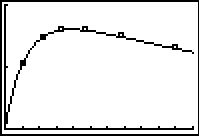
\includegraphics[width=2in]{./RationalsGraphics/CIRCRAT.jpg}}

\item The maximum power is approximately $1.603 \; mW$ which corresponds to $3.9 \; k\Omega$.

\item As $x \rightarrow \infty, \; P(x) \rightarrow 0^{+}$ which means as the resistance increases without bound, the power diminishes to zero.

\end{enumerate}

\end{enumerate}

\closegraphsfile